\documentclass[a4paper,
fontsize=11pt,
%headings=small,
oneside,
numbers=noperiodatend,
parskip=half-,
bibliography=totoc,
final
]{scrartcl}

\usepackage{synttree}
\usepackage{graphicx}
\setkeys{Gin}{width=.8\textwidth} %default pics size

\graphicspath{{./plots/}}
\usepackage[ngerman]{babel}
\usepackage[T1]{fontenc}
%\usepackage{amsmath}
\usepackage[utf8x]{inputenc}
\usepackage [hyphens]{url}
\usepackage{booktabs} 
\usepackage[left=2.4cm,right=2.4cm,top=2.3cm,bottom=2cm,headheight=25.60228pt,includeheadfoot]{geometry}
\usepackage{eurosym}
\usepackage{multirow}
\usepackage[ngerman]{varioref}
\setcapindent{1em}
\renewcommand{\labelitemi}{--}
\usepackage{paralist}
\usepackage{pdfpages}
\usepackage{lscape}
\usepackage{float}
\usepackage{acronym}
\usepackage{eurosym}
\usepackage[babel]{csquotes}
\usepackage{longtable,lscape}
\usepackage{mathpazo}
\usepackage[flushmargin,ragged]{footmisc} % left align footnote

%%url brekas grrr
\def\UrlBreaks{\do\a\do\b\do\c\do\d\do\e\do\f\do\g\do\h\do\i\do\j\do\k\do\l%
\do\m\do\n\do\o\do\p\do\q\do\r\do\s\do\t\do\u\do\v\do\w\do\x\do\y\do\z\do\0%
\do\1\do\2\do\3\do\4\do\5\do\6\do\7\do\8\do\9\do\-}%

\usepackage{listings}

\urlstyle{same}  % don't use monospace font for urls

\usepackage[fleqn]{amsmath}

%adjust fontsize for part

%% geometry
\clubpenalty = 10000 
\widowpenalty = 10000 
\displaywidowpenalty = 10000
%% tightlist

\providecommand{\tightlist}{%
  \setlength{\itemsep}{0pt}\setlength{\parskip}{0pt}}

\usepackage{sectsty}
\partfont{\large}

%Das BibTeX-Zeichen mit \BibTeX setzen:
\def\symbol#1{\char #1\relax}
\def\bsl{{\tt\symbol{'134}}}
\def\BibTeX{{\rm B\kern-.05em{\sc i\kern-.025em b}\kern-.08em
    T\kern-.1667em\lower.7ex\hbox{E}\kern-.125emX}}

\usepackage{fancyhdr}
\fancyhf{}
\pagestyle{fancyplain}
\fancyhead[R]{\thepage}

%meta

%meta

\fancyhead[L]{M. Hug, B.Fiechter \& Chr. Thomas \\ %author
LIBREAS. Library Ideas, 29 (2016). % journal, issue, volume.
\href{http://nbn-resolving.de/urn:nbn:de:kobv:11-100238186
}{urn:nbn:de:kobv:11-100238186}} % urn
\fancyhead[R]{\thepage} %page number
\fancyfoot[L] {\textit{Creative Commons BY 3.0}} %licence
\fancyfoot[R] {\textit{ISSN: 1860-7950}}

\title{\LARGE{Texte über fallende Steine. Alexander von Humboldts Praktiken wissenschaftlichen Arbeitens am Beispiel der \enquote{Mondvulkane}
}} %title %title
\author{Marius Hug, Benjamin Fiechter \& Christian Thomas} %author

\setcounter{page}{}

\usepackage[colorlinks, linkcolor=black,citecolor=black, urlcolor=blue,
breaklinks= true]{hyperref}

\date{}
\begin{document}

\maketitle
\thispagestyle{fancyplain} 

%abstracts

%body
\section*{Intro}\label{intro}

Am Abend des 16. Juni 1794 waren in Siena Steine vom Himmel gefallen.
Schnell hatte man eins und eins zusammengezählt: Die Steine mussten vom
Vesuv stammen. Dort, in rund 380 km Entfernung, hatte es tags zuvor eine
sehr starke Eruption gegeben. Hätte ein Stein mit einem Gewicht von 1 kg
bei Neapel mit einer Anfangsgeschwindigkeit v\textsubscript{0} und einem
Abschusswinkel $\alpha$ die Erdoberfläche verlassen, so wäre er tatsächlich am
nächsten Abend in der Toskana gelandet. Mathematisch besehen war diese
Hypothese also realistisch, und zwar spätestens seit Galilei
Berechnungen einer (idealen) Flugbahn (ohne Störungen wie sie
beispielsweise der Luftwiderstand mit sich brachte) angestellt
hatte.\footnote{\enquote{Man hat beobachtet, dass Wurfgeschosse eine
  gewisse Curve beschreiben; dass letztere aber eine Parabel sei, hat
  Niemand gelehrt.} (Vgl. Galilei 1891: 1). Um bei einer Entfernung von
  380 km eine Parabel zu beschreiben -- was einer störungsfreien
  Flugbahn entsprechen würde -- müssten die Steine eine Höhe von 95 km
  erreichen. Vgl. auch Tata 1800: 163, wobei dort wird in Meilen
  gerechnet.} Realistischer jedenfalls als die Annahme, es könnten
tatsächlich Steine buchstäblich vom Himmel gefallen sein. An
mittelalterliche Ansichten über Meteoriteneinschläge als Strafe Gottes
wollte man zum Ende des 18. Jahrhunderts in der Regel nicht mehr so
recht glauben.

Die Erklärung überzeugte aber eben nur mathematisch. Denn die
geophysikalischen Untersuchungen, die dem als \enquote{Steinregen von
Siena} in die Geschichte eingegangenen Naturschauspiel unmittelbar
folgten, zeigten recht schnell, dass die Steine nicht vom Vesuv stammen
konnten.\footnote{Siehe bspw. Vauquelin 1803: 37. Chemische Untersuchen
  finden sich bspw. bei Howard 1803: 293f.} Eine andere Theorie musste
her und diese fand man in der Vorstellung, dass es sich zwar durchaus um
Steine aus Vulkanausbrüchen handeln würde, doch nicht von Vulkanen auf
der Erde sondern von solchen auf dem Mond. So war damals die Rede von
Meteorsteinen selenitischer Herkunft.

\section*{\texorpdfstring{Kosmos-Vorträge über
\enquote{Meteorsteine}}{Kosmos-Vorträge über Meteorsteine}}\label{kosmos-vortruxe4ge-uxfcber-meteorsteine}

Am 15.4.1828, also 34 Jahre nach diesem ‚event`, referierte Alexander
von Humboldt in einem Hörsaal der Berliner Universität genau zu diesem
Thema: \enquote{Von den Meteorsteinen}, und zwar in der 53. Sitzung
seiner heute so genannten Kosmos-Vorträge.\footnote{Für das
  Wintersemester 1827/28 wurden im Lektionskatalog der Berliner
  Universität, der heutigen Humboldt-Universität, in der Sektion
  \enquote{Philosophische Wissenschaften} werden Humboldts Vorlesungen
  als Vorträge über \enquote{\emph{Physische Erdbeschreibung}, mit
  Prolegomenen über Lage, Gestalt und Naturbeschaffenheit der Gestirne}
  angekündigt. (Zit. nach Virmond 2011: 484. Hervorhebung im Original.)}
Bei diesen handelte sich um zwei teilweise parallel verlaufende
Vorlesungszyklen: Humboldt hat einmal an der Universität vor etwa 400
Hörern\footnote{Vgl. Virmond 2011: 484.} und einmal für ein noch
breiteres Publikum im damals größten überhaupt zur Verfügung stehenden
Vortragssaal, dem der Singakademie, vor immerhin 800 bis 1000\footnote{Vgl.
  Dove 1872: 143.} Zuhörern gelesen. Die Vorträge galten aufgrund der
hohen Besucherzahlen sowie der großen Aufmerksamkeit, die diese bereits
zeitgenössisch erfuhren, als \enquote{das bedeutendste gesellschaftliche
Ereignis Berlins dieser Jahre}\footnote{Lund 2012: 366; vgl. z. B. auch
  Werner 2004: 17.} und als \enquote{Sternstunden in der Geschichte der
Wissenschaftspopularisierung}.\footnote{Zit. Hamel; Tiemann 1993: 11
  vgl. ebd. sowie z. B. Daum 1998: 270--273.} Von dieser Veranstaltung
haben wir heute verschiedene Zeugnisse, da mehrere Nachschriften von
Zuhörern seiner Vorlesungen erhalten sind. Alle bisher bekannten
Nachschriften wurden und werden im Rahmen des Projekts \enquote{Hidden
Kosmos -- Reconstructing Alexander von Humboldt's ‚Kosmos-Lectures`} am
Institut für Kulturwissenschaft unter der Leitung von Christian Kassung
digitalisiert und im Volltext erfasst.\footnote{Das Projekt
  \enquote{Hidden Kosmos}
  (\url{http://www.culture.hu-berlin.de/hidden-kosmos}) wird in der
  Förderlinie \enquote{Freiräume} aus Mitteln der Exzellenzinitiative
  der Humboldt-Universität zu Berlin gefördert.}

Kommen wir nun zurück zu den vom Himmel fallenden
\enquote{Meteorsteinen} und steigen für einen kurzen Moment in die
entsprechende Passage der besagten 53. Vorlesung Humboldts ein (hier
zitiert aus der Nachschrift von G. Parthey):

\begin{quote}
Über die Ursachen des Phänomenes hat man 3 Hypothesen: 1, dass sich die
Steine in der Athmosphäre der Erde bilden {[}\ldots{}{]}. 2, dass sie
aus den Mondvulkanen hergeschleudert werden. {[}\ldots{}{]} 3, und dies
ist das wahrscheinlichste, dass die Steine im Weltraume selbst
herumfliegen {[}\ldots{}{]}\footnote{Parthey 1828: Bl. 336, , in:
  Deutsches Textarchiv
  \url{http://www.deutschestextarchiv.de/parthey_msgermqu1711_1828/675},
  abgerufen am 28.03.2016.}
\end{quote}

Uns interessiert die Mondvulkanhypothese, wenn sie auch nach Humboldt
nicht die wahrscheinlichste war. Konzentrieren wir uns also auf die
Mondvulkanhypothese und zitieren ohne Auslassung aus derselben
Nachschrift:

\begin{quote}
Poisson hat berechnet, dass eine Wurfkraft von 7100 Fus in der 1ten
Sekunde dazu gehört um die Steine vom Monde auf die Erde zu schleudern:
also 4 mal stärker als eine Kanonenkugel. Laplace fand, dass auf diese
Art ein Stein in 2½ Tagen zu uns kommen könne: allein Olbers bewies mit
musterhaftem Scharfsinn, dass Laplace dabei nicht auf die Translazion
des Mondes gerechnet habe, und dass, wenn man diese in Anschlag bringt,
die Steine aus den Mondvulkanen Erdsatelliten werden würden. Im Jahre
1660 wurde in Mayland ein Franziskanermönch durch einen Meteorstein
getödtet, wie der Physiker Tortona berichtet, und schon um dieselbe Zeit
1660, sagte Turzago in einem Mémoire darüber: dass der Stein aus dem
Monde gekommen sei.
\end{quote}

Nicht weniger als fünf Quellen (Poisson, Laplace, Olbers, Tortona,
Turzago) ruft Humboldt in seiner Vorlesung im Jahr 1828 auf, um seinen
Zuhörern diese Hypothese verständlich zu machen.\footnote{Bereits 1794
  ist sich Chladni sicher, dass es sich bei den Meteorsteinen nicht um
  tellurische, sondern um kosmische handeln muss (vgl. Chladni 1803:
  321). Allerdings lässt er auch 1803 die Entscheidung darüber offen, ob
  es sich dabei wirklich um kosmischen, oder doch eher selenitischen
  Ursprung handeln muss. Chladni wagt es (noch) nicht, Laplace zu
  widersprechen.} Um Missverständnisse zu vermeiden: Humboldt ist
sicherlich kein Anhänger der Mondvulkanhypothese. Aber offensichtlich
sind die Konsequenzen für ein Gesamtes der Erdanschauung wie auch die
damit verknüpften Namen und Werke so groß, dass sie nicht einfach
übergangen werden können.

So stellt sich die Frage: Welches Wissen stand Alexander von Humboldt
zur Verfügung? Wie sah seine Bibliothek, seine, wenn man so will,
Literaturdatenbank aus? Als wichtigstes Zeugnis der Bücher aus Humboldts
Privatbibliothek steht uns heute der \enquote{Catalogue of the Humboldt
Library} zur Verfügung (im Folgenden nach dem Verfasser Henry Stevens
auch als Stevens-Katalog bezeichnet). Der Großteil der Bücher wurde nach
Humboldts Tod durch einen Lagerhausbrand kurz vor der geplanten
Versteigerung bei Sotheby's vernichtet.\footnote{Vgl. Erdmann/Weber
  2015, Fußnote 35.} Zu Laplace finden sich im Auktionskatalog mit den
Nr. 5669--5672 vier Einträge, wobei vor allem die ersten drei
(\enquote{Précis de l'Histoire de l'Astronomie}, \enquote{Traité de
Mécanique céleste} und \enquote{Exposition du Systéme du Monde})
entsprechende Berechnungen über Meteorsteine enthalten könnten. Von
Olbers war die \enquote{Abhandlung über die Cometenbahn} in Humboldts
Besitz sowie dessen Briefwechsel mit F. W. Bessel. Die Nr. 7864--7868
entfallen auf Poisson, wobei hier sicherlich letzteres mit dem Titel
\enquote{Recherches sur le Mouvement des Projectiles dans l'Air} von
Interesse ist. Allerdings finden sich weder für Tortona noch für Turzago
irgendwelche Nachweise in diesem überlieferten Verzeichnis.

In einer anderen im \enquote{Hidden Kosmos} Projekt bearbeiteten
Vorlesungsnachschrift wird die Passage zu den Mondvulkanen im großen und
ganzen bestätigt mit dem feinen Unterschied, dass es nicht Tortona,
sondern Tortana heißt: \enquote{Im Jahre 1660 wurde ein Franziskaner
Mönch durch einen Meteorstein getödtet, und Tortana war der erste der
bei dieser Gelegenheit in einer kleinen Dissertation sagte, daß sie aus
dem Monde kämen.}\footnote{{[}N. N.{]} 1828a: 485, in: Deutsches
  Textarchiv
  \url{http://www.deutschestextarchiv.de/nn_oktavgfeo79_1828/491},
  abgerufen am 29.03.2016.} Zu diesem Tortana findet sich (im XML der
Transkription) eine editorische Anmerkung:

\begin{scriptsize}
\begin{verbatim}
<note resp="#BF" type="editorial">
    Vgl. <bibl>
    Terzago, Paolo Maria: Musaeum Septalianum Manfredi Septalae: 
             Patritii Mediolanensis Industrioso Labore constructum. Tortona 1664, 
             insbesondere Kapitel XVIII (S. 43–48).
    Online verfügbar: 
    <ref target="http://reader.digitale-sammlungen.de/de/fs1/object/display/bsb10051296_00075.html">
        MDZ München, abgerufen am 29.02.2016.
    </ref>
</bibl>
</note>
\end{verbatim}
\end{scriptsize}

Editorische Notizen dieser Art wurden im Projekt \enquote{Hidden Kosmos}
im Rahmen einer Bachelorarbeit in die Projektdaten
eingepflegt.\footnote{Darauf wird später noch ausführlich eingegangen
  werden.} Die Notiz ist hier insofern interessant, da sich plötzlich
die Verwirrung um Tortona oder Tortana und Turzago auflöst. Alles war
irgendwie falsch, denn richtig wäre gewesen, dass es sich um eine
Publikation eines Paola Maria Terzago handelt, mit Tortona dagegen keine
Person, sondern der Verlagsort gemeint war.

Was aber heißt im Kontext von Vorlesungsnachschriften falsch und
richtig? Hatte Humboldt sich geirrt? Oder wurde er schlicht
missverstanden? Glücklicherweise liegen neben den Nachschriften der
Universitätsvorlesungen auch noch zwei Nachschriften des
Singakademie-Zyklus' vor.\footnote{An der Singakademie hat Humboldt
  seine Vorlesungen über physikalische Geographie mit gleichem
  Themenumfang in nur 16 Vorträgen gehalten, an der Universität waren es
  62.}

In der Nachschrift von Otto Hufeland hat dieser die entsprechende
Passage wie folgt festgehalten:

\begin{quote}
Bei der versuchten Erklärung dieses Phänomens haben einige die
Behauptung aufgestellt, daß die herabgeschleuderten Massen Producte der
Mondvulkane wären {[}\ldots{}{]}. La Place und Olbers haben die Frage
aufgeworfen, welche Wurfkraft erforderlich sein würde, um einen
dergleichen Auswurf bis in die Attractionssphäre unserer Erde zu
bringen. Mathematische Rechnungen ergeben, daß eine schwere Masse, die
aus dem Monde mit einer anfänglichen Geschwindigkeit von 7500′ in 1
Secunde, ungefähr die vierfache Geschwindigkeit einer Kanonenkugel,
geschleudert würde, nach 2½ Tagen auf unserer Erde anlangen könnte
{[}\ldots{}{]} Uebrigens ist diese Meinung nicht neu, und schon Paulo
Maria Torzago in Tortosa hat die Vermuthung geäussert, daß die
Steinregen aus dem Monde herabkommenn möchten.\footnote{Hufeland 1829:
  144, in: Deutsches Textarchiv
  \url{http://www.deutschestextarchiv.de/hufeland_privatbesitz_1829/148},
  abgerufen am 29.03.2016.}
\end{quote}

Bereits diese Querverbindung innerhalb der Projektdaten hätte sicherlich
genügt, um die entsprechende Quelle -- die hier ja immerhin schon Person
und Ort beinhaltete -- über eine simple Literaturrecherche ausfindig zu
machen und mit unseren Daten zu verlinken. Wobei dieser Arbeitsschritt
in zweierlei Hinsicht einen Mehrwert für das Projekt bedeutet:
Einerseits um die zwar aufgerufene, aber unvollständig ausgewiesene
Quelle kenntlich zu machen, und andererseits, um diese Quelle im
Folgenden in eine Gesamtbibliographie der in den
\enquote{Kosmos-Vorlesungen} zitierten Werke einzupflegen.

Aufgrund der Einbettung von \enquote{Hidden Kosmos} in das Deutsche
Textarchiv an der Berlin-Brandenburgischen Akademie der Wissenschaften
steht uns aber ein weit größeres Korpus zur Verfügung.\footnote{Die
  Nachschriften werden sukzessive im Deutschen Textarchiv (DTA) der
  Berlin-Brandenburgischen Akademie der Wissenschaften (BBAW)
  veröffentlicht:
  \url{http://www.deutschestextarchiv.de/search/metadata?corpus=avhkv}.
  Zusätzlich stehen die XML-Volltexte, verschiedene daraus extrahierte
  Übersichten (bspw. eine Übersicht der in den Vorlesungen erwähnten
  Personen oder Instrumente) sowie die im Projekt entwickelten Skripte
  auf GitHub online: \url{https://github.com/haoess/hidden-kosmos}.}
Dort finden sich mittlerweile über 2400 digitalisierte Werke in XML/TEI,
in der Regel nach den Erstveröffentlichungen und ein Großteil davon aus
dem 19. Jahrhundert. So verwundert es nicht, dass dort neben den fünf
\emph{Kosmos}-Bänden Alexander von Humboldts weitere 167 Werke desselben
Autors zur Verfügung stehen.\footnote{Neben einer wachsenden Anzahl von
  unselbstständigen Schriften stehen im DTA auch zahlreiche Werke von
  Humboldts Zeitgenossen zur Verfügung. Alle Texte A. v. Humboldts im
  DTA unter www.deutschestextarchiv.de/api/pnd/118554700; zu den Korpora
  der unselbstständigen Schriften Humboldts und seiner Vorträge an der
  Königlich Preußischen Akademie siehe Thomas 2015a und 2015b.}
Erweitern wir also unser Suchmuster auf alle Werke des Autors Alexander
von Humboldt, werden wir tatsächlich im ersten Band des \emph{Kosmos}
von 1845 fündig:

\begin{quote}
Wenn man indeß den ganzen Umfang der Verhältnisse erwägt, die ich schon
in diesem Naturgemälde habe aufzählen müssen, um dem Verdacht
unbegründeter Behauptungen zu entgehen, so findet man die Hypothese des
selenitischen Ursprunges der Meteorsteine von einer Mehrzahl von
Bedingungen abhängig, deren zufälliges Zusammentreffen allein das bloß
Mögliche als ein Wirkliches gestalten kann. Einfacher und anderen
Vermuthungen über die Bildung des Sonnensystems analoger scheint die
Annahme eines ursprünglichen Daseins kleiner planetarischer Massen im
Weltraume.\footnote{Humboldt 1845: 127, in: Deutsches Textarchiv
  \url{http://www.deutschestextarchiv.de/humboldt_kosmos01_1845/146},
  abgerufen am 29.03.2016.}
\end{quote}

In der dazugehörigen dreiseitigen(!) Endnote ruft Humboldt neben den
bereits bekannten Akteuren um Laplace, Olbers, Terzago wichtige
Argumente auf, die gegen die Hypothese von den Mondvulkanen
sprechen.\footnote{Daneben gibt er den Hinweis, dass es unter den
  \enquote{griechischen Physikern} (genannt werden bspw. Diogenes,
  Plinius, Anaxagoras, Euripides und natürlich Aristoteles) die gängige
  Meinung gab, dass die Steine von der Sonne stammen könnten. Der
  selenitische Ursprung, also Steine vom Mond, spielte bei den Griechen
  noch keine Rolle.} Da es sich hierbei vornehmlich um ballistische
Berechnungen handelt, das heißt um Berechnungen unter welcher
Anfangsgeschwindigkeit die \enquote{Geschosse} den Mond verlassen haben
müssten und auf welcher Flugbahn sie dann in die Erdatmosphäre
eindringen würden, könnte man zusammenfassend sagen: Die Mathematik
sprach für, die Physik aber gegen Mondvulkane.

Die vielen Quellen, die Humboldt im ersten Band seines \emph{Kosmos}
(1845) anführt und von denen viele bereits Gegenstand der Vorlesungen
von 1827/28 war, lassen auf einen umfangreiches und avanciertes
Ordnungssystem schließen, in dem Humboldt die einschlägigen
bibliographischen Daten für die jeweils behandelten Themen organisierte.
In der Tat wurde erst 2009 von Dominik Erdmann und Christian Thomas im
Nachlass A. v. Humboldts eine Sammlung von Zetteln entdeckt, die
eindeutig den Kosmos-Vorträgen zuzuordnen sind.\footnote{Vgl. Dove 1872:
  425f; zur (Wieder-)Auffindung dieser Manuskripte Erdmann/Thomas 2010
  und dies. 2014, bes.: 39--42.} Bis zum heutigen Datum kann die
Existenz dieser Manuskripte, die Humboldt selbst in der Vorrede zum
ersten Band des \emph{Kosmos} vehement bestritt,\footnote{Vgl. Humboldt
  1845: X.} als der Forschung weitestgehend unbekannt gelten.

Diese, im Nachlass Humboldts in der Berliner Staatsbibliothek SBB-PK
aufbewahrten, eigenhändigen Vortragsmanuskripte wurden von Humboldt
selbst über viele Jahre hinweg für verschiedene Publikationen genutzt.
Dabei sind sie teilweise zerschnitten, um späteres Wissen erweitert und
innerhalb der Systematik seiner ‚Kollektaneen zum \emph{Kosmos`} neu
geordnet worden.\footnote{Vgl. Thomas/Erdmann 2014: 36 und 41f. Sowie
  jüngst Erdmann/Weber 2015: 60--62.} Auf einem dieser Zettel geht es
unter anderem um Mondvulkane (siehe Abb. 1). In der Bildmitte heißt es
etwa: \enquote{Meteorsteine II. Mondvulcane können uns Steine lancieren
wenn min 7500 F par seconde Lapl 2-3 T}:\footnote{A. v. Humboldts
  Handschrift ist mitunter, wie unschwer zu erkennen, nicht einfach zu
  transkribieren. An dieser Stelle gebührt Dominik Erdmann Dank, der
  hier zu Rate gezogen werden konnte.}

\begin{figure}[htbp]
\centering
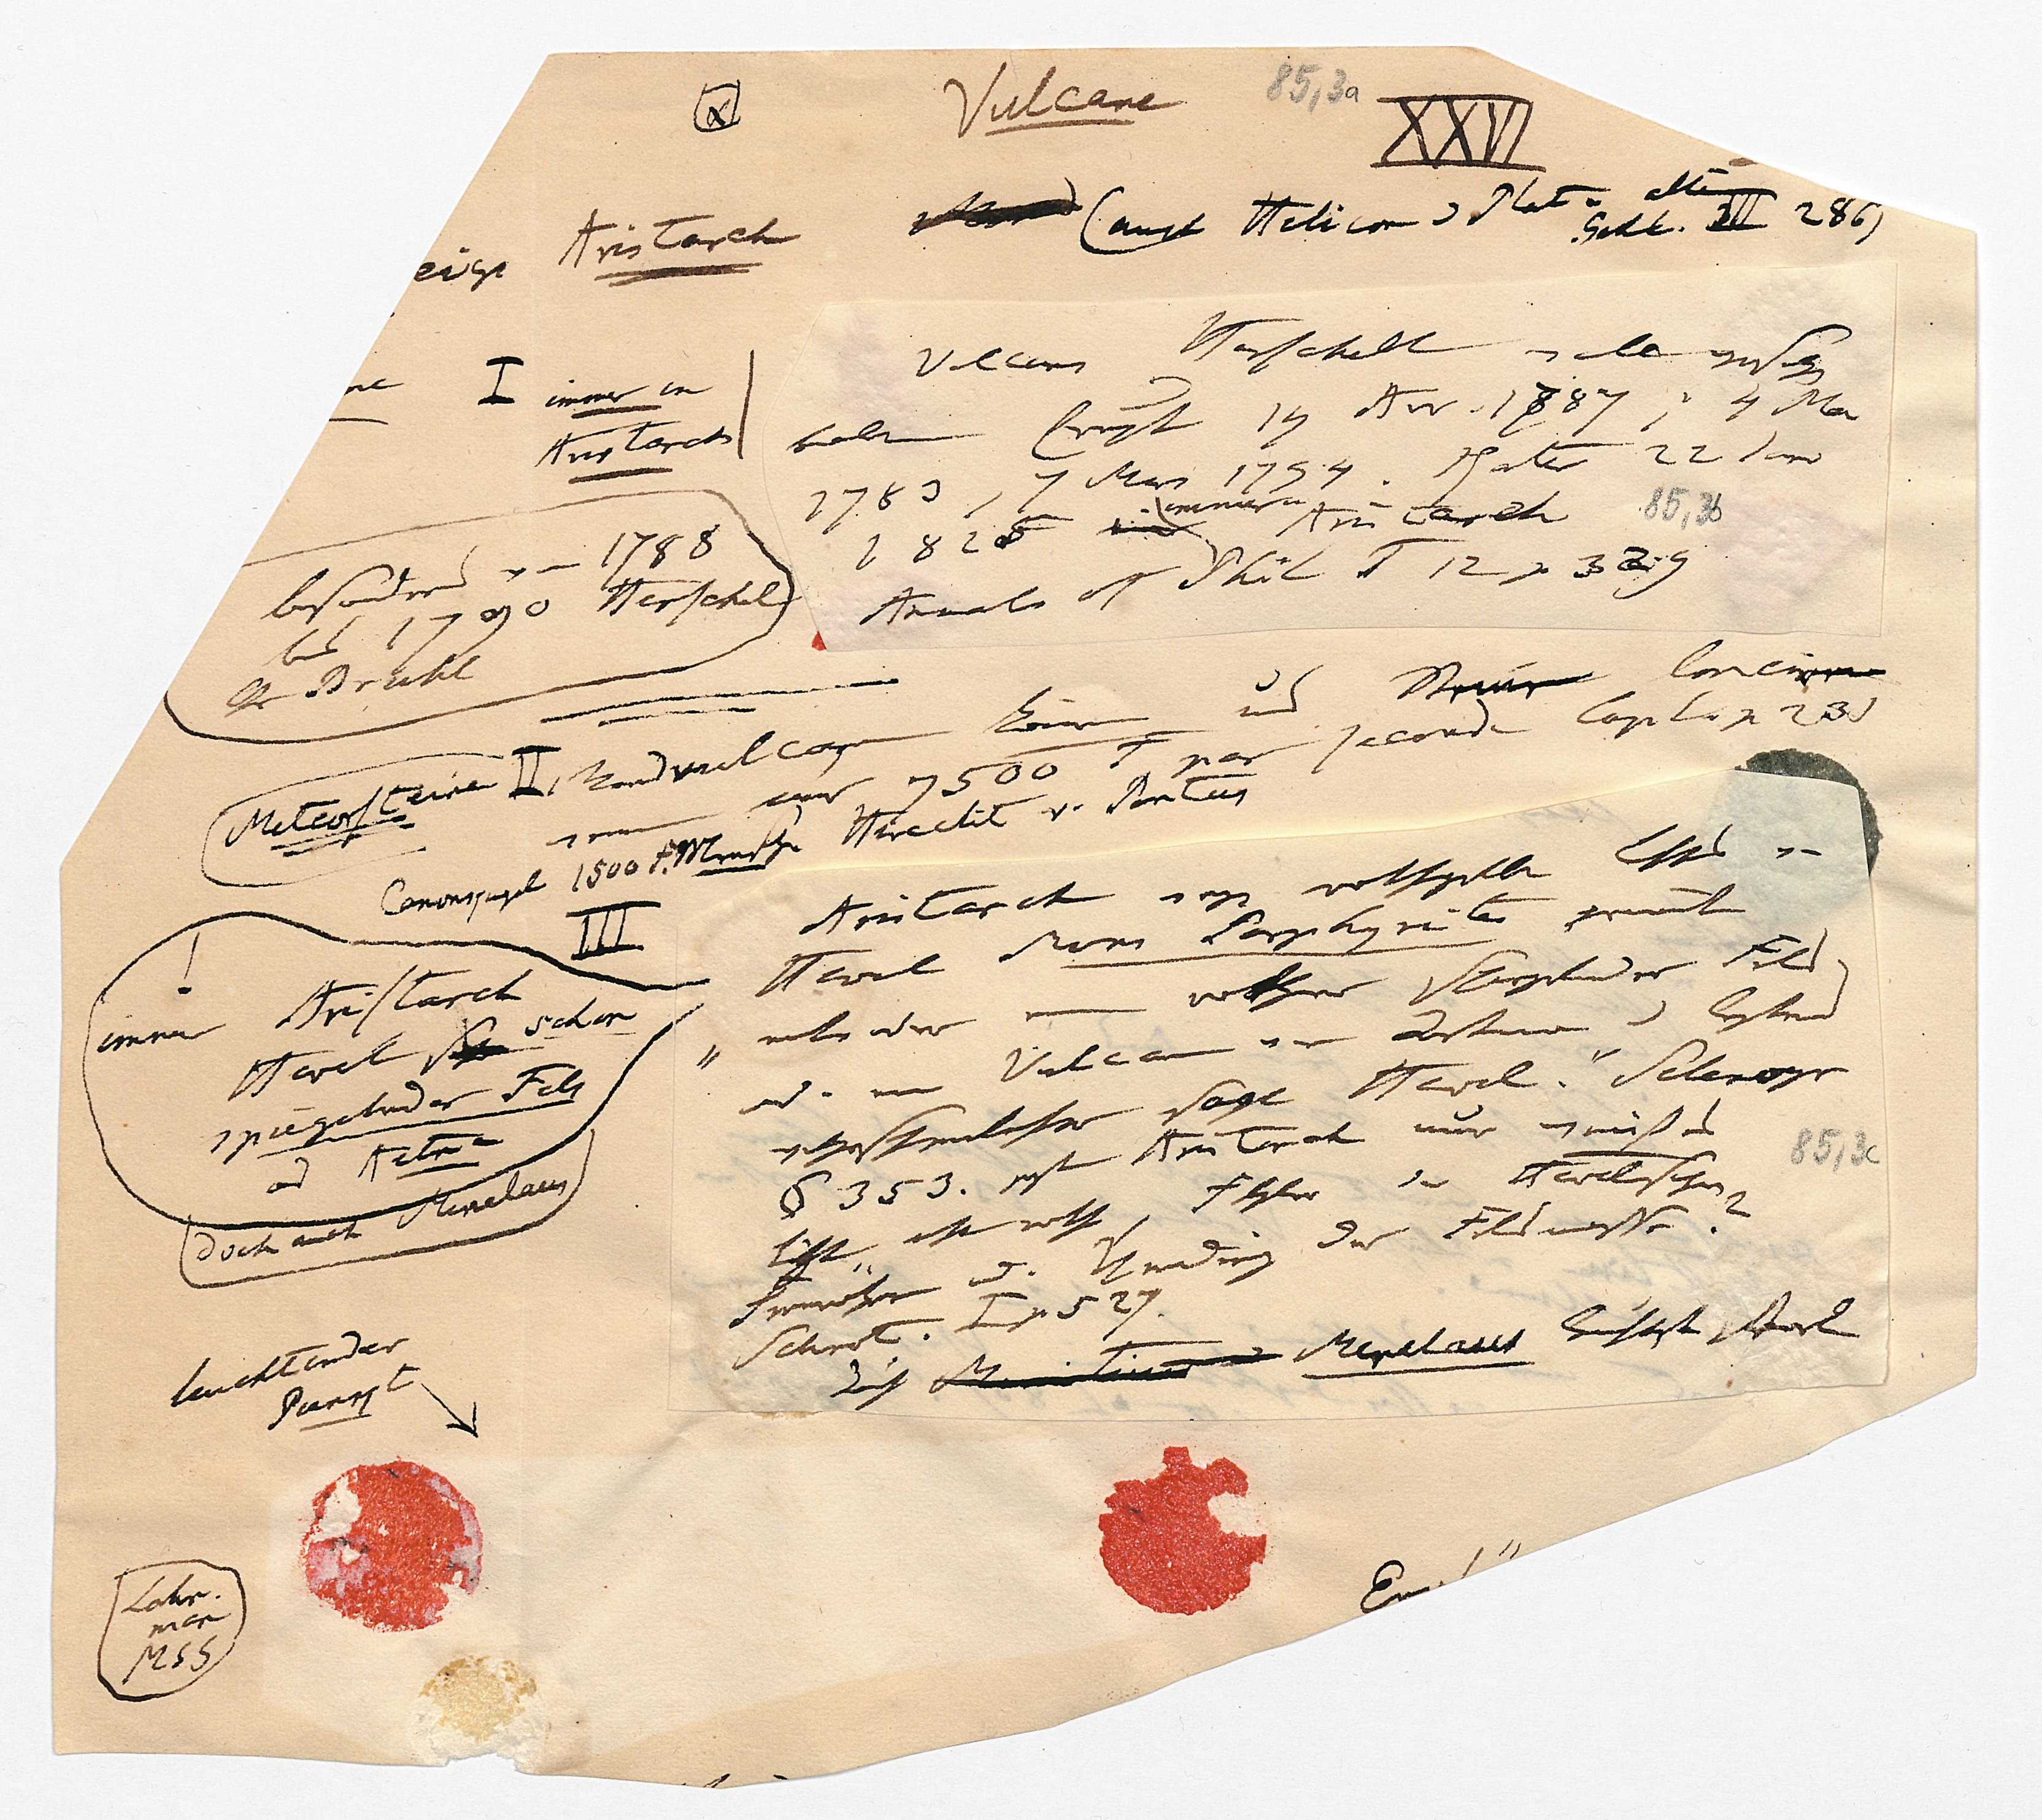
\includegraphics{img/01.jpg}
\caption{Originalmanuskript Humboldts aus dem Nachlass an der
Staatsbibliothek zu Berlin -- Preußischer Kulturbesitz (SBB-PK): Nachl.
Alexander von Humboldt, kl. Kasten 3b, Nr. 85, Bl. 3r.
\url{http://resolver.staatsbibliothek-berlin.de/SBB00018C4E00000009}.}
\end{figure}

Das Vorhandensein dieser Information (mit nur geringfügigen
grammatikalischen Anpassungen) sowohl in der Vorlesungsnachschrift von
Otto Hufeland\footnote{Wie Anm. 15.} wie auch im ersten Band von
Humboldts \emph{Kosmos}\footnote{Humboldt 1845: 400, Fußnote 39.} , kann
als Indiz gedeutet werden, dass dieser Zettel an beiden Ereignissen Teil
hatte.

\section*{Zwischenbemerkung}\label{zwischenbemerkung}

Am Beispiel der Meteorsteine konnten wir einen Einblick in die
Arbeitstechniken A. v. Humboldts geben. In Humboldts Werk, der sich vor
allem im \emph{Kosmos} mit nicht weniger als dem \emph{Ganzen} -- was
alle Phänomene in den \enquote{irdischen und himmlischen
Räumen}\footnote{Humboldt 1847: 249.} mit einschließt --
auseinandersetzte, war der Verweis auf die entsprechenden Quellen (das
kann man der Fülle von Anmerkungen im Endnotenapparat
entnehmen\footnote{Auf die Bedeutung dieses zweigeteilten Designs,
  Haupttext plus Anmerkungen, geht Humboldt im zweiten Band des
  \emph{Kosmos} ein: \enquote{Es ist der Zweck der Anmerkungen zum
  Kosmos, nicht etwa bloß bibliographische Quellen aus verschiedenen
  Litteraturen zur Erläuterung dessen darzubieten, was im Texte
  behauptet wird; ich habe in diesen Anmerkungen, die eine freiere
  Bewegung gestatten, auch einen reichhaltigen Stoff des Nachdenkens
  niederlegen wollen, so wie ich ihn aus der Erfahrung und aus langen
  litterarischen Studien habe schöpfen können.} (Vgl. Humboldt 1847:
  420, FN 59). Zu dieser geschachtelten Konstruktion wiederum bemerkt
  Christian Bermes treffend: \enquote{Daß diese Anmerkungsanmerkung
  selbst eine Anmerkung in und zu einer Anmerkung ist, darf als ein
  geglücktes Spiel angesehen werden, das die Ebenenverschmelzung von
  Inhalt und Beschreibung noch einmal verdeutlicht.} (Vgl. Bermes 2004,
  82, FN 222).}) von zentraler Bedeutung. In unserem Projekt des
\enquote{Reconstructing Alexander von Humboldts ‚Kosmos Lectures`} nimmt
die Bibliographie ebenfalls eine immens wichtige Rolle ein. Und genau
deshalb gilt es, sich den Herausforderungen zu stellen, die, wie oben
gezeigt, darin bestehen, dass 1) Humboldts Hörer nicht jede Referenz
korrekt und ausführlich notieren konnten; dass daher 2) oft nur mehrere
Vortragsnachschriften im Vergleich mit- und in Ergänzung zueinander dazu
führen, die Verweise zufriedenstellend auflösen zu können; und 3)
dadurch, dass unsere Quellen immer auch und vor allem Zeugnis einer
ursprünglich mündlichen Rede sind, in deren Verlauf die referierten
Gegenstände nicht immer in der Ausführlichkeit eines überbordenden
Quellenapparates à la \emph{Kosmos} behandelt werden konnten.\footnote{Für
  weitere Bespiele siehe Thomas/Fiechter/Hug 2016.}

Die Berechnungen der erforderlichen Geschwindigkeiten der vermeintlich
vom Mond stammenden Steine bezeugen genau das: Nur in Humboldts
\emph{Kosmos} ist Raum für die exakten Zahlen: Olbers errechnet 7780 Fuß
in der Secunde, Laplace 7377 F., Biot 7771 F. und Poisson 7123
F.\footnote{Humboldt 1845: 400, in: Deutsches Textarchiv
  \url{http://www.deutschestextarchiv.de/humboldt_kosmos01_1845/419},
  abgerufen am 29.03.2016.} In den Vorträgen dagegen wurde, wohl um der
besseren Verständlichkeit willen, auf 7500 Fuß gerundet, und sogar das
war keine Garantie dafür, dass Parthey daraus nicht 7100
machte.\footnote{Eine Suche über die Vorlesungsnachschriften im Bestand
  des Deutschen Textarchivs
  (\url{http://www.deutschestextarchiv.de/search/ddc}) zeigt, dass es
  sich dabei wirklich um eine Ausnahme handelte: /(7100\textbar{}7500)/
  \&\& /Se{[}ck{]}/ \#has{[}flags,/avhkv/{]}. Die 7100 findet sich nur
  in Partheys Nachschrift, in den anderen Nachschriften heißt es
  richtigerweise 7500.}

\begin{figure}[htbp]
\centering
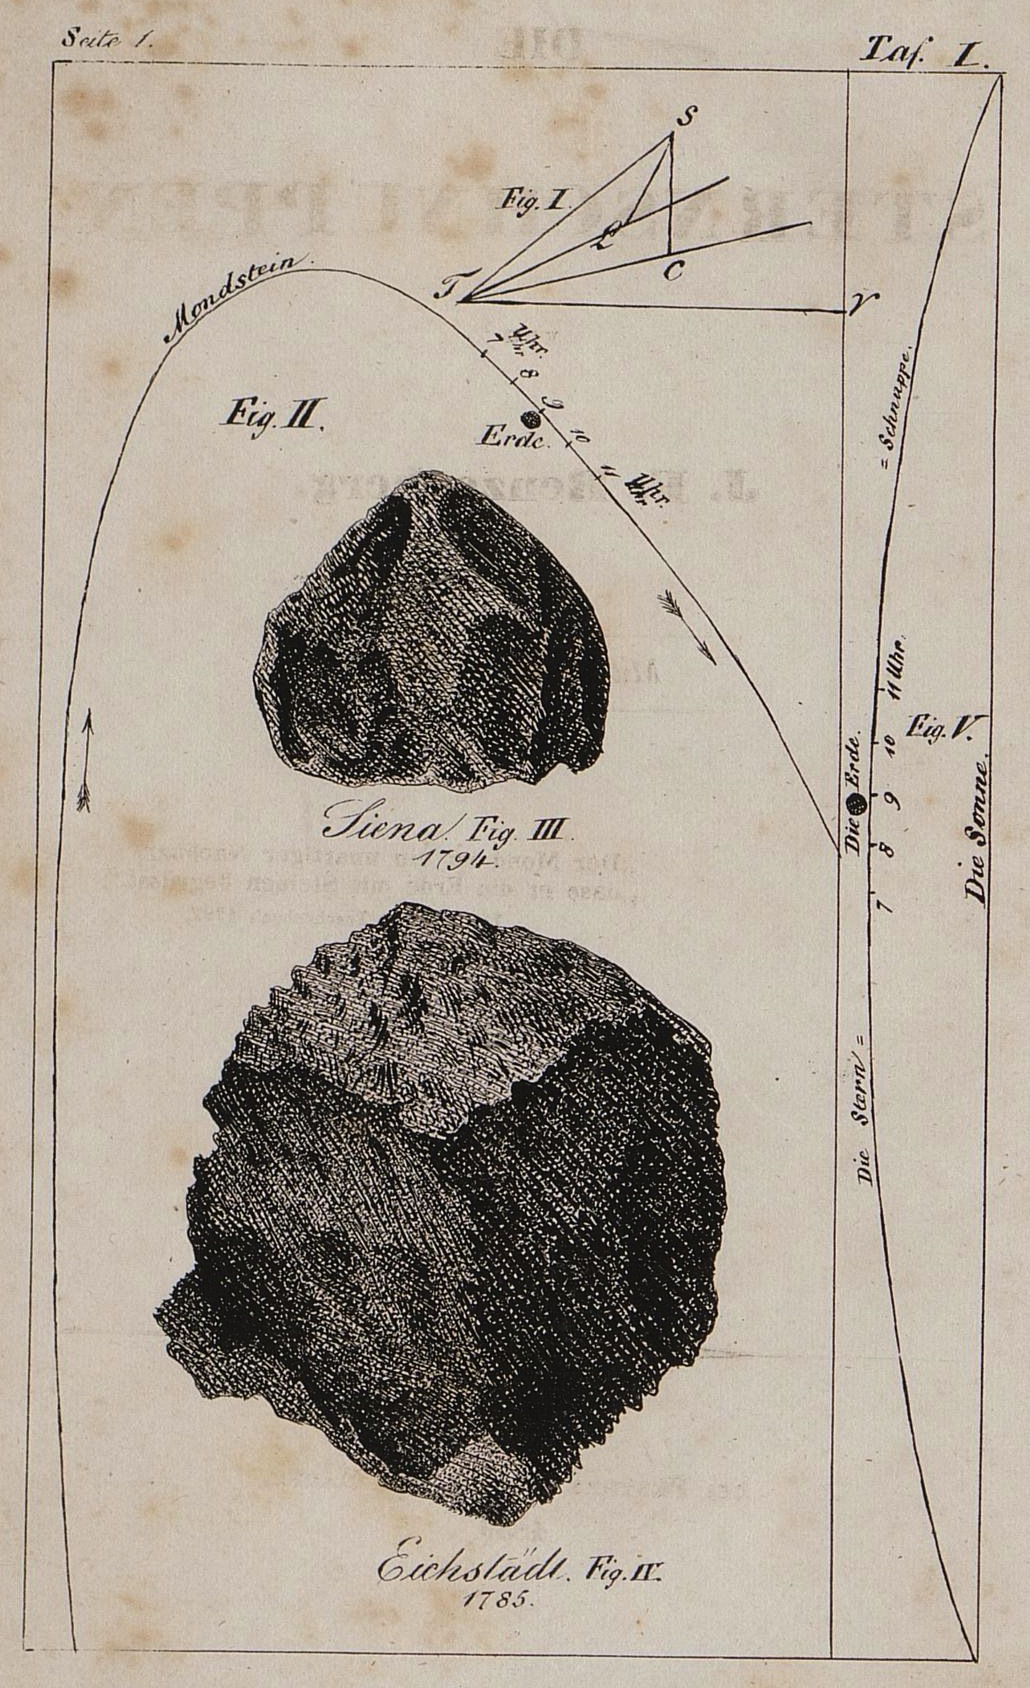
\includegraphics{img/02.jpg}
\caption{Darstellung eines angeblichen Mondsteins sowie der zugehörigen
Fallkurve aus Benzenberg 1839: Tafel 1}
\end{figure}

Umso wichtiger aber, dass die genannten Quellen recherchiert und
verlinkt werden. Und wenn das hier exemplarisch am Beispiel der
angeblich vom Mond fallenden Steine gezeigt wurde, so ist klar, dass die
Voraussetzung für weitere Untersuchungen dieser Art in einer
Gesamtbibliographie zu Alexander von Humboldts Kosmos-Vorträgen besteht.
Eine erste Version einer solchen \enquote{Liste der in den Nachschriften
zitierten, genannten und auf andere Weise referenzierten Werke} wurde
von November 2015 bis Januar 2016 von Benjamin Fiechter erstellt und als
Bachelorarbeit an der Humboldt-Universität zu Berlin eingereicht. Im
Folgenden soll auf die so entstandene Humboldt-Bibliographie näher
eingegangen werden.

\section*{Erstellung einer Bibliographie zu den
Kosmos-Vorträgen}\label{erstellung-einer-bibliographie-zu-den-kosmos-vortruxe4gen}

Angesichts des begrenzten Zeitraumes und der Anforderungen an eine
Bachelorarbeit im Fach Deutsche Literatur konnte nur ein Ausschnitt der
in den Kosmos-Vorträgen aufgerufenen Literatur recherchiert und
abgebildet werden. So entstanden 32 Seiten Bibliographie (von insgesamt
50 Seiten Bachelorarbeit) mit 87 Einträgen. Neben den eigentlichen
bibliographischen Angaben enthält die Bibliographie Verweise auf
Retrodigitalisate beziehungsweise Volltexte des jeweiligen Titels, eine
Überprüfung auf das Vorhandensein im Stevens-Katalog\footnote{Das
  Verzeichnis von Humboldts gesamter nachgelassener Bibliothek, s. o.}
sowie die Fundstellen in sechs der zehn bekannten Nachschriften, die zu
diesem Zeitpunkt bereits durch das Projekt \enquote{Hidden Kosmos}
veröffentlicht worden waren.

Problematisch war zu Beginn die Festlegung eines Formates für die
Aufnahme der bibliographischen Angaben. Dabei waren weder Regelwerke für
Bibliotheken noch international verbreitete Zitationsformate von Nutzen.
So erwiesen sich sowohl die Regeln für die alphabetische Katalogisierung
(in wissenschaftlichen Bibliotheken) (RAK-{[}WB{]})\footnote{Regeln für
  die alphabetische Katalogisierung in wissenschaftlichen Bibliotheken
  (RAK-WB), \url{http://d-nb.info/986402338/34}, abgerufen am
  29.03.2016.} als auch das neue internationale Regelwerk Resource
Description and Access (RDA)\footnote{RDA Steering Committee (RSC) for
  the Development of RDA: Resource Description and Access,
  \url{http://www.rda-jsc.org/archivedsite/rda.html}, abgerufen am
  29.03.2016.} als nicht geeignet, angesichts der Tatsache, dass in der
Regel eine Autopsie nötig gewesen wäre, um alle dort obligatorischen
Angaben zu ermitteln -- was im Rahmen einer Bachelorarbeit und auch im
Rahmen des \enquote{Hidden Kosmos}-Projekts nicht zu leisten war.
Umgekehrt sind insbesondere amerikanische Zitationsformate wie zum
Beispiel APA Style\footnote{American Psychological Association: APA
  Style, \url{http://www.apastyle.org/}, abgerufen am 29.03.2016.} oder
Harvard System of Referencing\footnote{Siehe Anglia Ruskin University
  Library -- Harvard System: Guide to the Harvard System of Referencing
  (5th edition):
  \url{http://libweb.anglia.ac.uk/referencing/harvard.htm}, abgerufen am
  29.03.2016.} zu allgemein und ungenau gehalten, um sie hierfür
einsetzen zu können. Letztlich wurden die Regeln des Instituts für
Deutsche Literatur der Humboldt-Universität zu Berlin in leicht
abgewandelter Form angewandt, außerdem orientiert an den Regeln des
Deutschen Textarchivs zur Metadatenaufnahme.\footnote{Deutsches
  Textarchiv (DTA): DTA-Basisformat -- Header,
  \url{http://deutschestextarchiv.de/doku/basisformat_header}, abgerufen
  am 29.03.2016.} Aufgrund der Entscheidung, in der Bachelorarbeit nur
einen Ausschnitt aus der später zu erstellenden Gesamtbibliographie zu
zeigen, konnten die priorisierten Titel dafür umso umfassender
recherchiert werden.\footnote{Ausgangspunkt waren die sogenannten
  \enquote{Quellen der Wissenschaft}, die sich in allen Nachschriften
  der Universitätsvorlesungen finden. Hier führte Humboldt eine Reihe
  von aus seiner Sicht besonders wichtigen, zeitgenössischen und
  historischen Werken auf, wobei die verschiedenen Hörer auch hier
  verschiedene Werke notiert haben. Darüber hinaus wurden einzelne
  Themenbereiche in den Fokus genommen, z. B. Literatur zu Mondbewohnern
  oder von Humboldt erwähnte Belletristik.}

Zuerst galt es, die oft falsch beziehungsweise gelegentlich völlig
entstellten Namen der Verfasser zu identifizieren (\enquote{Langeerde}
statt La Métherie;\footnote{{[}N. N.{]} 1828c: 39, in: Deutsches
  Textarchiv
  \url{http://www.deutschestextarchiv.de/nn_msgermqu2345_1827/45},
  abgerufen am 30.03.2016.} \enquote{Liston} statt Littrow,
\enquote{Foller} statt Vollmer\footnote{{[}N. N.{]} 1828d: 58, in:
  Deutsches Textarchiv
  \url{http://www.deutschestextarchiv.de/nn_n0171w1_1828/58}, abgerufen
  am 30.03.2016. Derzeit, stand März 2016, befindet sich dieser Text
  noch in DTAQ, der webbasierten Plattform zur Qualitätssicherung des
  DTA und ist daher nur nach Registrierung und Anmeldung zugänglich.}
oder \enquote{Hopfner} statt Hoff\footnote{{[}N. N.{]} 1828a: 63, in:
  Deutsches Textarchiv
  \url{http://www.deutschestextarchiv.de/nn_oktavgfeo79_1828/69},
  abgerufen am 30.03.2016.} et cetera). Bei den Identifizierungen der
Personen waren -- wie das oben am Beispiel der Mondvulkane bereits
gezeigt wurde -- die Parallelstellen der verschiedenen Nachschriften
sehr hilfreich, so dass nahezu alle Verweise, die einen Namen und eine
Schrift nennen, aufgelöst werden konnten. Problematisch sind nach wie
vor sowohl ungenaue Notizen, die nur in einem Manuskript vorhanden sind
(zum Beispiel \enquote{v. Halle{[}:{]} Welträume}\footnote{{[}N. N.{]}
  1828c: 40, in: Deutsches Textarchiv
  \url{http://www.deutschestextarchiv.de/nn_msgermqu2345_1827/46},
  abgerufen am 30.03.2016.} -- vermutlich ist hier Edmond Halley
gemeint, aber welches seiner Werke?), als auch von Humboldt bewusst
unscharf gehaltene Angaben: \enquote{Ein sonst geistreicher
Schriftsteller glaubte, um das Ueberkommen der reißenden Thiere zu
erklären, zu der Annahme genöthigt zu seyn, daß sie als ganz kleine
Thiere in denselben Böten{[}!{]}, worin die Menschen kamen, mit
eingeschifft worden wären.}\footnote{{[}N. N.{]} 1828b: 60v, in:
  Deutsches Textarchiv
  \url{http://www.deutschestextarchiv.de/nn_msgermqu2124_1827/124},
  abgerufen am 30.03.2016.} Der gemeinte Autor, der diese Hypothese
vertrat, konnte bislang nicht identifiziert werden.

In den meisten Fällen wurden nur unvollständige Namen, oft ohne
zugehöriges Werk, notiert. Hier musste mit der hypothetischen
Identifizierung des Autors zugleich ein thematisch passendes Werk
recherchiert werden.\footnote{Selbstverständlich bot es sich in einigen
  Fällen auch an, das gesuchte Werk über den Stevens-Katalog selbst zu
  identifizieren.} Besonderes Augenmerk wurde dabei auf Familien
gerichtet, deren Angehörige über mehrere Generationen hinweg
Forscherpersönlichkeiten hervorgebracht haben und häufig auch in
ähnlichen Feldern wissenschaftlich aktiv waren.

Standen der gesuchte Autor und das zugehörige Werk fest, wurde versucht,
diejenige Ausgabe zu ermitteln, die Humboldt selbst benutzte. In der
Regel ließ sich der Erscheinungszeitraum auf spätestens 1828 eingrenzen,
da die Kosmos-Vorträge in diesem Jahr endeten.\footnote{Da Humboldt auch
  auf noch unpublizierte Manuskripte verwies, sind einige wenige Werke
  in der Bibliographie enthalten, die erst später erschienen sind.}
Zunächst wurde im Stevens-Katalog nach einer passenden Ausgabe gesucht
(mehr als ein Viertel der Titel in der Bibliographie sind dort
aufgeführt); war dort keine passende Ausgabe zu finden, wurde im
\emph{Kosmos} (1845--1862) weitergesucht. Wenn auch hier keine genaueren
Angaben zu entnehmen waren, wurde auf die letzte, für Humboldt zu diesem
Zeitpunkt in Betracht kommende Ausgabe verwiesen, da Humboldt von vielen
Werken die neueste Ausgabe besaß, wie aus dem Stevens-Katalog
hervorgeht. Bei häufig verlegten Autoren wie zum Beispiel Dante, Cicero
oder Galilei stellte sich diese Herangehensweise als problematisch
heraus; eine gewisse Beliebigkeit bei der Ausgabenauswahl konnte hier
nicht vermieden werden. Erst jetzt konnte der Titel vollständig
bibliographisch aufgenommen werden.

Anschließend wurde nach einem frei zugänglichen Bilddigitalisat der
ermittelten Ausgabe gesucht. Waren mehrere Digitalisate derselben
Ausgabe verfügbar, war das wichtigste Kriterium bei der Auswahl die
Qualität der Scans, außerdem wurde die verantwortliche Institution
berücksichtigt, weil etwa bei Google Books ein dauerhafter Zugriff nicht
garantiert ist.

Schließlich wurden die bibliographischen Angaben sowie URLs zum
Digitalisat in den zugehörigen XML-Dateien der Nachschriften als
Anmerkungen eingefügt. Sie ermöglichen es dem Leser, unmittelbar auf die
Quelle der zuvor genannten Information zuzugreifen. Die Zusammenführung
im Sinne einer umfassenden Übersicht wird zurzeit vorbereitet und
spätestens mit Auslaufen der Projektförderung im August 2016 auf der
projekteigenen Webseite verfügbar sein.\footnote{Siehe
  www.culture.hu-berlin.de/hidden-kosmos. Neben der Bereitstellung einer
  Online-Übersicht der Bibliographie ist ein zur weiteren Verarbeitung
  herunterladbares Format (BibTeX, RIS) in Planung.} An der
Bibliographie wird kontinuierlich weitergearbeitet, so dass eine
möglichst vollständige Auflistung entsteht.

\section*{Schlussbemerkung}\label{schlussbemerkung}

Abschließend soll ein alternativer -- man könnte sagen deduktiver --
Zugriff wenigstens angedeutet werden: In den Kosmos-Vorlesungen fehlt
mit dem deutschen Physiker und Geometer Johann Friedrich Benzenberg eine
wichtige Referenz zum Thema Sternschnuppen (eine Visualisierung von
diesem, die unter anderem den Steinregen von Siena thematisiert, ist in
Abbildung 2 dargestellt). Benzenberg veröffentlichte bereits 1801 in den
Annalen der Physik erste Beobachtungen von Sternschnuppen.\footnote{Benzenberg
  1801: 370--374.} In den 1830er Jahren publizierte er erneut wichtige
Schriften zum Thema und war bemerkenswerterweise nach wie vor ein
Verfechter der Mondvulkanhypothese.

Diese in den 1830er Jahren veröffentlichten Werke Benzenbergs wurden von
Alexander von Humboldt zur Kenntnis genommen, was nicht zuletzt die
Eintragungen im Stevens-Katalog belegen, und haben eindeutig Eingang in
den \emph{Kosmos} gefunden. Dieser Befund führt auf Fragen zur
Arbeitsweise Humboldts, die sich ausgehend von der hier vorgestellten
Bibliographie der Kosmos-Vorträge zumindest zum Teil werden beantworten
lassen: 1) Welche Zeitschriften hat Humboldt regelmäßig zur Kenntnis
genommen? Es findet sich beispielsweise im gesamten zur Verfügung
stehenden Korpus kein einziger expliziter Beleg, dass Humboldt mit dem
\enquote{Polytechnischen Journal}\footnote{http://dingler.culture.hu-berlin.de}
gearbeitet hätte, obwohl es mit dieser Referenz in Sachen Publikation
technischer Fortschritte thematisch viele Überschneidungen gäbe. 2) Mit
welchen Kriterien der Selektion arbeitete Humboldt, wenn er Benzenberg
einerseits für eine \enquote{scharfsinnige Bemerkung}\footnote{Humboldt
  1859: 58, in: Deutsches Textarchiv
  \url{http://www.deutschestextarchiv.de/humboldt_aequinoktial02_1859/66},
  abgerufen am 31.03.2016.} und generell seine \enquote{verdienstvollen
Bemühungen}\footnote{Humboldt 1850: 592, in: Deutsches Textarchiv
  \url{http://www.deutschestextarchiv.de/humboldt_kosmos03_1850/599},
  abgerufen am 31.03.2016.} lobt, andererseits aber seiner (noch Anfang
der 1830er Jahre in Teilen vertretenen\footnote{Darauf, dass die
  Geschichte -- wie immer -- noch viel komplizierter sein kann, sei hier
  exemplarisch hingewiesen: Benzenberg revidiert die Hypothese, dass
  alle Meteorsteine vom Mond stammen, teilweise. Anfang der 1830er Jahre
  lässt sich eine Periodizität -- also eine jährliche Wiederholung -- im
  Erscheinen von Sternschnuppen nicht mehr leugnen. Diese macht aber
  freilich keinen Sinn, wenn die Steine direkt vom Mond zur Erde
  geschleudert werden. Benzenberg ging also fortan von zwei
  unterschiedlichen Klassen von Meteorsteinen aus, nämlich periodischen
  und nichtperiodischen. Siehe dazu die präzisen Untersuchungen von
  Schwarz 2014: 39--50, v. a. 44f.}) Mondvulkanhypothese längst
widerspricht? Daran anschließend 3): Lässt sich anhand der Nachschriften
durchgängig belegen, dass Humboldt in seinen Vorträgen diejenigen
Forscher ganz bewusst namentlich unerwähnt lässt, deren Hypothesen er
für Unsinn hält\footnote{Siehe dazu das oben aufgeführte Beispiel der
  Theorie eines nicht namentlich genannten \enquote{sonst
  geistreiche{[}n{]} Schriftsteller{[}s{]}}, dass die reißenden Tiere
  sozusagen als Miniaturversionen mit den Booten der Einwanderer auf den
  amerikanischen Kontinent gelangt seien.} -- um also seine Hörer gerade
nicht zur Lektüre von deren Arbeiten zu (ver-)führen?

Humboldts Faszination für Sternschnuppen und Meteorsteine scheint
besonders ausgeprägt. Wenn aber nur \enquote{eine ununterbrochene und
systematisch fortgesetzte Beobachtung}\footnote{Humboldt, Alexander von
  (1851): 27.} zu einer Erklärung dieser Phänomene führen kann, so muss
diese Vorgehensweise beinahe sinnbildlich auf Humboldts gesamtes
Schaffen übertragen werden. Und die Herausforderungen, die eine
Ermittlung der expliziten und impliziten Literaturverweise in den
Kosmos-Vorträgen Humboldts, dessen dazugehörigen Manuskripten aus dem
Nachlass und deren Zusammenführung in einer umfassenden Bibliographie
mit sich bringt, erfordern ein ebenso ununterbrochenes und
systematisches Arbeiten im \enquote{Hidden Kosmos} - Projekt, um
letztendlich zu einer möglichst vollständigen Übersicht über Humboldts
Quellen gelangen zu können.

\section*{Bibliographie}\label{bibliographie}

\begin{itemize}
\item
  Anonymus (1797): \enquote{Steinregen zu Siena}. \emph{Göttinger
  Taschen Calender \textgreater{} für das Jahr 1797}, 161--69.
  Göttingen: Joh. Chr. Dieterich.
\item
  Benzenberg, Johann Friedrich (1801): \enquote{Beobachtungen von
  Sternschnuppen.} \emph{Annalen Der Physik} 9: 370--74.
\item
  Benzenberg, Johann Friedrich (1839): \emph{Die Sternschnuppen: Mit 9
  Steintafeln}. Hamburg: Perthes.
\item
  Bermes, Christian (2004): \emph{Welt Als Thema Der Philosophie: Vom
  Metaphysischen Zum Natürlichen Weltbegriff}. Meiner Verlag.
\item
  Chladni, Ernst Florens Friedrich (1794): \emph{Ueber den Ursprung der
  von Pallas gefundenen und anderer ihr ähnlicher Eisenmassen (etc.)}.
  Riga: Johann Friedrich Hartknoch.
\item
  Chladni, Ernst Florens Friedrich (1803): \enquote{Chronologisches
  Verzeichniss der mit einem Feuermeteor niedergefallenen Stein- und
  Eisenmassen, nebst einigen Bemerkungen}. \emph{Annalen der Physik} 15
  (11): 307--28.
\item
  Daum, Andreas W. (1998): \emph{Wissenschaftspopularisierung im 19.
  Jahrhundert. Bürgerliche Kultur, naturwissenschaftliche Bildung und
  die deutsche Öffentlichkeit 1848--1914}. München: Oldenbourg
  Wissenschaftsverlag.
\item
  Dove, Alfred (1872): \enquote{Alexander von Humboldt auf der Höhe
  seiner Jahre. (Berlin 1827--59.)}, in: Bruhns, Karl (Hg.):
  \emph{Alexander von Humboldt: Eine wissenschaftliche Biographie}. 3
  Bde. Leipzig: Brockhaus, Bd. 2., S. 93--484.
\item
  Erdmann, Dominik; Christian Thomas (2010): \enquote{Aussicht vom
  Zettelgebirge -- Zur Datenverarbeitung in Alexander von Humboldts
  Manuskripten der Kosmos-Vorlesungen}, in: \emph{Trajekte} 20, S.
  30--36.
\item
  Erdmann, Dominik; Christian Thomas (2014): \enquote{›\ldots{} zu den
  wunderlichsten Schlangen der Gelehrsamkeit zusammengegliedert‹. Neue
  Materialien zu den ›Kosmos-Vorträgen‹ Alexander von Humboldts, nebst
  Vorüberlegungen zu deren digitaler Edition}. \emph{HiN. Internationale
  Zeitschrift für Humboldt-Studien} 15 (28): 34--45.
\item
  Erdmann, Dominik; Jutta Weber (2015): \enquote{Nachlassgeschichten --
  Bemerkungen zu Humboldts nachgelassenen Papieren in der Berliner
  Staatsbibliothek und der Biblioteka Jagiellonska Krakau}. \emph{HiN.
  Internationale Zeitschrift für Humboldt-Studien} 16 (31): 58--77.
\item
  Gehler, Johann Samuel Traugott (1837): \enquote{Meteorstein}.
  \emph{Gehler's Physikalisches Wörterbuch} 6 (3): 2084--2152.
\item
  Hamel, Jürgen; Klaus-Harro Tiemann (Hg.) (1993): \emph{Alexander von
  Humboldt: Über das Universum. Die Kosmosvorträge 1827/28 in der
  Berliner Singakademie}. Frankfurt a. M.: Insel.
\item
  Howard, H. Ed. (1803): \enquote{Versuche und Bemerkungen über Stein-
  und Metallmassen, die zu verschiedenen Zeiten auf die Erde gefallen
  seyn solten, und über die gediegnen Eisenmassen}. \emph{Annalen der
  Physik} 13: 291--327.
\item
  Hufeland, Otto (1829): Vorlesungen über physicalische Geographie von
  A. v. Humboldt. {[}G{]}eschrieben im Sommer 1829 durch Otto Hufeland.
  {[}Berlin{]}, {[}ca. 1829{]}. {[}= Nachschrift der
  \enquote{Kosmos-Vorträge} Alexander von Humboldts in der Sing-Akademie
  zu Berlin, 6.12. 1827--27.3.1828{]} In: Deutsches Textarchiv
  \url{http://www.deutschestextarchiv.de/hufeland_privatbesitz_1829},
  abgerufen am 30.03.2016.
\item
  Humboldt, Alexander von (1845): Kosmos. Entwurf einer physischen
  Weltbeschreibung. Bd. 1. Stuttgart u. a. In: Deutsches Textarchiv
  \url{http://www.deutschestextarchiv.de/humboldt_kosmos01_1845},
  abgerufen am 30.03.2016.
\item
  Humboldt, Alexander von (1847): Kosmos. Entwurf einer physischen
  Weltbeschreibung. Bd. 2. Stuttgart u. a. In: Deutsches Textarchiv
  \url{http://www.deutschestextarchiv.de/humboldt_kosmos02_1847},
  abgerufen am 30.03.2016.
\item
  Humboldt, Alexander von (1850): Kosmos. Entwurf einer physischen
  Weltbeschreibung. Bd. 3. Stuttgart u. a. In: Deutsches Textarchiv
  \url{http://www.deutschestextarchiv.de/humboldt_kosmos03_1850},
  abgerufen am 30.03.2016.
\item
  Humboldt, Alexander von (1851): \emph{Atlas Zu Alexander v. Humboldt's
  Kosmos in Zweiundvierzig Tafeln Mit Erläuterndem Texte}. Hrsg. von
  Traugott Bromme. Stuttgart: Krais \& Hoffmann.
  \url{http://www.biodiversitylibrary.org/item/89025}.
\item
  Humboldt, Alexander von (1859): Reise in die Aequinoktial-Gegenden des
  neuen Kontinents. Bd. 2. Übers. v. Hermann Hauff. Stuttgart. In:
  Deutsches Textarchiv
  \url{http://www.deutschestextarchiv.de/humboldt_aequinoktial02_1859},
  abgerufen am 31.03.2016.
\item
  Laplace, Pierre Simon (1824): \emph{Exposition du système du monde}.
  5ème ed. Paris: Bachelier.
  \url{http://hdl.handle.net/2027/mdp.39015065834759}.
\item
  Lund, Hannah Lotte (2012): \enquote{Die Universität in der Stadt
  1810--1840. Geselligkeit -- Kultur -- Politik}, in: Heinz-Elmar
  Tenorth und Charles McClelland (Hg.): \emph{Geschichte der Universität
  Unter den Linden}, Bd 1: \emph{Gründung und Blütezeit der Universität
  zu Berlin, 1810--1918}. Berlin: Akademie Verlag, S. 325--380.
\item
  {[}N. N.{]} (1828a): Die physikalische Geographie von Herrn Alexander
  v. Humboldt, vorgetragen im Semestre 1827/28. {[}Berlin{]},
  {[}1827/28{]}. {[}= Nachschrift der \enquote{Kosmos-Vorträge}
  Alexander von Humboldts in der Berliner Universität,
  3.11.1827--26.4.1828{]} In: Deutsches Textarchiv \url{http://www.deutschestextarchiv.de/nn_oktavgfeo79_1828}, 
  abgerufen am 30.\\03.2016.
\item
  {[}N. N.{]} (1828b): Physikalische Geographie. Vorgetragen von
  Alexander von Humboldt. {[}Berlin{]}, {[}1828{]}. {[}= Nachschrift der
  \enquote{Kosmos-Vorträge} Alexander von Humboldts in der Sing-Akademie
  zu Berlin, 6.12.1827--27.3.1828{]} In: Deutsches Textarchiv
  \url{http://www.deutschestextarchiv.de/nn_msgermqu2124_1827},
  abgerufen am 31.03.2016.
\item
  {[}N. N.{]} (1828c): Alexander von Humboldts Vorlesungen über
  phÿsikalische Geographie nebst Prolegomenen über die Stellung der
  Gestirne. Berlin im Winter von 1827 bis 1828. {[}Berlin{]},
  {[}1827/28{]}. {[}= Nachschrift der \enquote{Kosmos-Vorträge}
  Alexander von Humboldts in der Berliner Universität,
  3.11.1827--26.4.1828{]} In: Deutsches Textarchiv
  \url{http://www.deutschestextarchiv.de/nn_msgermqu2345_1827},
  abgerufen am 31.03.2016.
\item
  {[}N. N.{]} (1828d): Physikalische Geographie von Heinr. Alex.
  Freiherr v. Humboldt. {[}V{]}or\-ge\-tra\-gen im Wintersemester 1827/8.
  {[}Berlin{]}, {[}1827/28{]}. {[}= Nachschrift der
  \enquote{Kosmos-Vor\-träge} Alexander von Humboldts in der Berliner
  Universität, 3.11.1827--26.4.1828{]} In: Deutsches Textarchiv \\
  \url{http://www.deutschestextarchiv.de/dtaq/book/view/nn_n0171w1_1828},
  abgerufen am 30.03.2016.
\item
  Olbers, Heinrich Wilhelm (1837): \enquote{Die Sternschnuppen}.
  \emph{Jahrbuch für 1837}, herausgegeben von Heinrich Christian
  Schumacher, 36--64.
\item
  Parthey, Gustav (1828): Alexander von Humboldt{[}:{]} Vorlesungen über
  physikalische Geographie. Novmbr. 1827 bis April,{[}!{]} 1828.
  Nachgeschrieben von G. Partheÿ. {[}Berlin{]}, {[}1827\\/28{]}. {[}=
  Nachschrift der \enquote{Kosmos-Vorträge} Alexander von Humboldts in
  der Berliner Universität, 3.11.1827--26.4.1828{]} In: Deutsches
  Textarchiv
  \url{http://www.deutschestextarchiv.de/parthey_msgermqu1711_1828},
  abgerufen am 30.03.2016.
\item
  Schwarz, Oliver (2014): \enquote{Alexander von Humboldt als
  astronomischer Arbeiter, Diskussionspartner und Ideengeber}.
  \emph{HiN. Internationale Zeitschrift für Humboldt-Studien} 15, Nr.
  29: 39--50.
\item
  Tata, Abbé Domenico (1800): \enquote{Ueber den Steinregen zu Siena am
  16ten Juni 1794.} \emph{Annalen Der Physik} 6: 156--69.
\item
  Terzago, Paolo Maria und Manfredi Settala (1664): \emph{Musaeum
  Septalianum Manfredi Septalae patritii Mediolanensis industrioso
  labore constructum}. Typis filiorum qd. Elisei Violae.
\item
  Thomas, Christian (2015a): \enquote{99 unselbständige Schriften
  Humboldts als Volltext im Deutschen Textarchiv verfügbar}, in:
  \emph{avhumboldt.de, Alexander von Humboldt Informationen online},
  \url{http://www.avhumboldt.de/?p=10922}.
\item
  ­Thomas, Christian (2015b): \enquote{Humboldts Akademie-Abhandlungen
  als Volltext im Deutschen Textarchiv veröffentlicht}. In:
  \emph{avhumboldt.de, Alexander von Humboldt Informationen online},
  \url{http://www.avhumboldt.de/?p=10959}.
\item
  Thomas, Christian; Benjamin Fiechter und Marius Hug (2016):
  \enquote{Methoden und Ziele der Erschließung handschriftlicher Quellen
  zu Alexander von Humboldts Kosmos-Vorträgen: Das Projekt Hidden
  \emph{Kosmos} der Humboldt-Universität zu Berlin.} Erscheint in:
  Horizonte der Humboldtforschung, hrsg. v. Ottmar Ette und Julian
  Drews. Hildesheim: Olms-Weidmann, 2016. PREPRINT-Verison unter
  \url{https://www.culture.hu-berlin.de/de/forschung/projekte/hidden-kosmos/media/thomas-fiechter-hug-2016-04-03-preprint.pdf}.
\item
  Vauquelin, Louis-Nicolas (1803): \enquote{Verhandlungen, die Analyse
  und den Ursprung meteorischer Stein- und Metallmassen betreffend.
  Abhandlung über die angeblich vom Himmel gefallenen Steine}. Übersetzt
  von Gehlen. \emph{Neues allgemeines Journal der Chemie} 1 (1): 37--51.
\item
  Virmond, Wolfgang (Hg.) (2011): \emph{Die Vorlesungen der Berliner
  Universität 1810--1834 nach dem deutschen und lateinischen
  Lektionskatalog sowie den Ministerialakten}. Berlin: Akademie Verlag.
\item
  Werner, Petra (2004): \emph{Himmel und Erde. Alexander von Humboldt
  und sein Kosmos}. Berlin: Akademie Verlag.
\end{itemize}

%autor
\begin{center}\rule{0.5\linewidth}{\linethickness}\end{center}

\textbf{Marius Hug} hat von 2000--2006 an der Humboldt-Universität zu
Berlin Kulturwissenschaft und Philosophie studiert. Er war von
2007--2009 wissenschaftlicher Mitarbeiter im Forschungsprojekt
``Geschichte der technischen Bildübertragung (1843--1923)'' an der
Universität Konstanz und assoziiertes Mitglied des Zukunftskollegs. Von
01--07/2008 war er zudem Stipendiat am ``Center for Knowledge
Architecture'' an der TU Dresden. Von 2009--2013 koordinierte er das von
der DFG geförderte Projekt ``Digitalisierung des Polytechnischen
Journals'' (\url{http://www.polytechnischesjournal.de}). Von 2013--2015
war er Koordinator des weiterbildenden Masterstudiengangs
Psychoanalytische Kulturwissenschaft an der Humboldt-Universität zu
Berlin und ist seither wissenschaftlicher Mitarbeiter im aus Mitteln der
Exzellenz-Initiative geförderten Projekt ``Hidden Kosmos: Reconstructing
A. v. Humboldt's ›Kosmos-Lectures‹''
(\url{http://www.culture.hu-berlin.de/hidden-kosmos}).

\textbf{Benjamin Fiechter} studiert seit 2011 an der
Humboldt-Universität zu Berlin Deutsche Literatur und Geschichte, seit
2015 im Masterstudiengang Deutsche Literatur. Er war studentische
Hilfskraft im DFG-geförderten Projekt ``Deutsches Textarchiv'' (DTA,
\url{http://www.deutschestextarchiv.de}). Seit 2014 arbeitet er im
Projekt ``Hidden Kosmos: Reconstructing A. v. Humboldt's ›Kosmos-Lectures‹''
(\url{http://www.culture.hu-berlin.de/hidden-kosmos}), gefördert aus
Mitteln der Exzellenz-Initiative, als studentische Hilfskraft. Außerdem
ist er aktiver Beiträger der freien Quellensammlung ``Wikisource''
(Wikimedia Foundation, \url{https://de.wikisource.org/}).

\textbf{Christian Thomas} hat Neuere deutsche Literatur und Philosophie
an der Humboldt-Universität zu Berlin studiert und ist seit 2010
wissenschaftlicher Mitarbeiter im DFG-geförderten Projekt ``Deutsches
Textarchiv'' (DTA, www.deutschestextarchiv.de) und im Projekt
``CLARIN-D'' (\url{http://www.clarin-d.de}) an der
Berlin-Brandenburgischen Akademie der Wissenschaften. Im Rahmen von
CLARIN-D koordinierte er ein Kurationsprojekt zur Aufwertung und
Integration historischer Textressourcen des 15.--19. Jahrhunderts in die
Korpora des DTA bzw. von CLARIN-D
(\url{http://www.deutschestextarchiv.de/clarin_kupro}). Seit Juni 2014
koordiniert er zudem als wissenschaftlicher Mitarbeiter der
Humboldt-Universität zu Berlin das aus Mitteln der Exzellenz-Initiative
geförderte Projekt ``Hidden Kosmos: Reconstructing
A. v. Humboldt's ›Kosmos-Lectures‹''
(\url{http://www.culture.hu-berlin.de/hidden-kosmos}). Parallel dazu arbeitet
er an einer Promotion über die bislang größtenteils unveröffentlichten
Nachschriften der ``Kos\-mos\-Vorlesungen'' Alexander von Humboldts.

\end{document}